\documentclass[11pt]{article}
\usepackage{geometry,marginnote} % Pour passer au format A4
\geometry{hmargin=1cm, vmargin=1cm} % 

% Page et encodage
\usepackage[T1]{fontenc} % Use 8-bit encoding that has 256 glyphs
\usepackage[english,french]{babel} % Français et anglais
\usepackage[utf8]{inputenc} 

\usepackage{lmodern,numprint}
\setlength\parindent{0pt}

% Graphiques
\usepackage{graphicx,float,grffile,units}
\usepackage{tikz,pst-eucl,pst-plot,pstricks,pst-node,pstricks-add,pst-fun,pgfplots} 

% Maths et divers
\usepackage{amsmath,amsfonts,amssymb,amsthm,verbatim}
\usepackage{multicol,enumitem,url,eurosym,gensymb,tabularx}

\DeclareUnicodeCharacter{20AC}{\euro}



% Sections
\usepackage{sectsty} % Allows customizing section commands
\allsectionsfont{\centering \normalfont\scshape}

% Tête et pied de page
\usepackage{fancyhdr} \pagestyle{fancyplain} \fancyhead{} \fancyfoot{}

\renewcommand{\headrulewidth}{0pt} % Remove header underlines
\renewcommand{\footrulewidth}{0pt} % Remove footer underlines

\newcommand{\horrule}[1]{\rule{\linewidth}{#1}} % Create horizontal rule command with 1 argument of height

\newcommand{\Pointilles}[1][3]{%
  \multido{}{#1}{\makebox[\linewidth]{\dotfill}\\[\parskip]
}}

\newtheorem{Definition}{Définition}

\usepackage{siunitx}
\sisetup{
    detect-all,
    output-decimal-marker={,},
    group-minimum-digits = 3,
    group-separator={~},
    number-unit-separator={~},
    inter-unit-product={~}
}

\setlength{\columnseprule}{1pt}

\begin{document}

\textbf{Nom, Prénom :} \hspace{8cm} \textbf{Classe :} \hspace{3cm} \textbf{Date :}\\

\begin{center}
  \textit{Il faut apprendre, non pas pour l'amour de la connaissance, mais pour se défendre contre le mépris dans lequel le monde tient les ignorants.}  - \textbf{Charlie Chaplin}
\end{center}

\subsection*{ex1 - Méthode 1 : Produit en croix}
\textit{Les tableaux sont proportionnels.} \newline
\textbf{Écrire les calculs et calculer.}

\begin{multicols}{4}\noindent
  \begin{center}
    \begin{tabular}{|c|c|}
      \hline
      1 & 32\\  \hline
      14,5 & $\phantom{azertyuiop}$\\  \hline
    \end{tabular}
  \end{center}
  \Pointilles[1]
  \begin{center}
    \begin{tabular}{|c|c|}
      \hline
      12 & $\phantom{azertyuiop}$\\  \hline
      1,5 & 24\\  \hline
    \end{tabular}
  \end{center}
  \Pointilles[1]
  \begin{center}
    \begin{tabular}{|c|c|}
      \hline
      $\phantom{azertyuiop}$  & 24\\  \hline
      8 & 68\\  \hline
    \end{tabular}
  \end{center}
  \Pointilles[1]
  \begin{center}
    \begin{tabular}{|c|c|}
      \hline
      12 & 46\\  \hline
      $\phantom{azertyuiop}$ & 24\\  \hline
    \end{tabular}
  \end{center}
  \Pointilles[1]
\end{multicols}

\begin{center}
  \begin{tabular}{|c|c|c|c|c|c|}
    \hline
   3 &  3,1                   &                  45000 &  \phantom{100 000 000} &  \phantom{100 000 000} &                     9\\ \hline
   7 &  \phantom{100 000 000} &  \phantom{100 000 000} &                   7400 &                    0,4 &  \phantom{100 000 000}\\ \hline     
  \end{tabular}
\end{center}
\Pointilles[5]

\subsection*{ex2 - Méthode 2 : Proportionnel ?}
\textit{Les tableaux sont-ils proportionnels ? } \newline
\textbf{Écrire les calculs et une phrase réponse.}

\begin{minipage}[t]{0.2\textwidth}
  \begin{enumerate}
    \item[1.]
    \begin{tabular}{|c|c|c|}
      \hline
      24 & 96 & 212 \\  \hline
      2 & 8 & 26\\  \hline
    \end{tabular}
  \item[2.]
    \begin{tabular}{|c|c|c|}
      \hline
      12 & 18 & 6 \\  \hline
      30 & 45 & 15\\  \hline
    \end{tabular}
  \end{enumerate}
\end{minipage}
\begin{minipage}[t]{0.8\textwidth}
  \Pointilles[6]
\end{minipage}

\begin{minipage}[t]{0.45\textwidth}
  \subsection*{ex3 - Tableur}

  \begin{enumerate}
    \item[1.] Quel nombre est dans la case : \textbf{C5} ? \dotfill
    \item[2.] Quelle case a pour nombre : \textbf{18} ? \dotfill
  \end{enumerate}

\end{minipage}
\begin{minipage}[t]{0.5\textwidth}

  \begin{figure}[H]
        \centering
        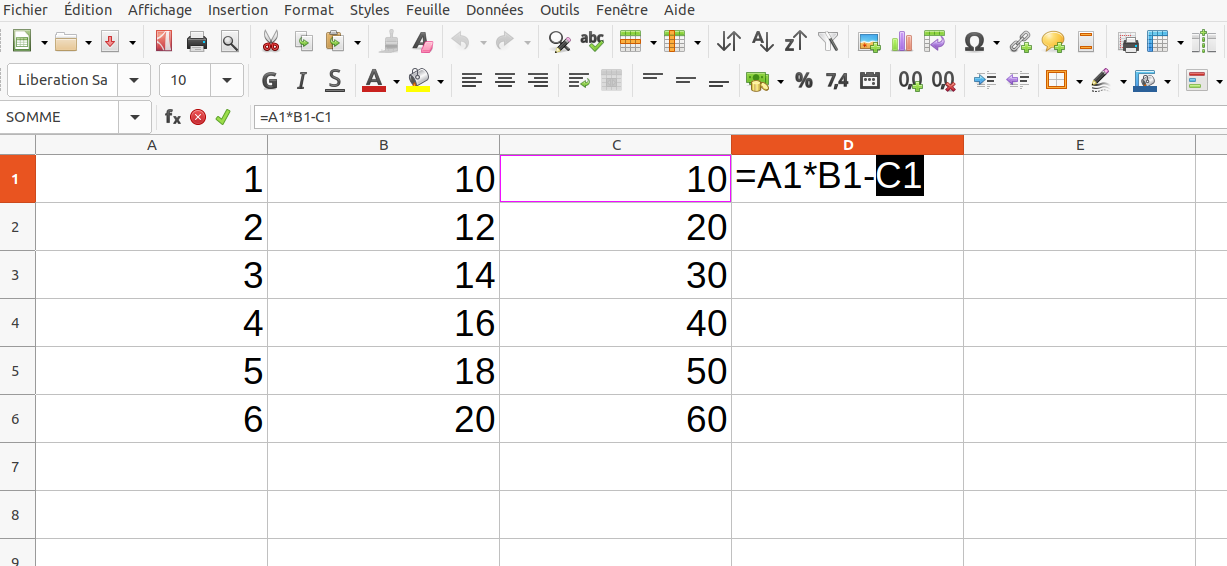
\includegraphics[width=\linewidth]{4x2-proportionnalite/ie-tableur.png}
  \end{figure}

\end{minipage}

\begin{enumerate}
  \item[3.] Quel nombre sera affiché dans la case \textbf{B7} après avoir \textbf{étiré} le tableau vers le bas ? \dotfill
  \item[4.] Quel nombre sera affiché dans la case \textbf{D2} après avoir \textbf{étiré} la formule de la case D1 ? \dotfill
  \item[5.] Quelle formule écrire dans la case \textbf{E2} pour faire le calcul : $(12-2) \times 20$ ? \dotfill
\end{enumerate}

\newpage

\subsection*{ex4 - Des petits problèmes}
\textit{Il faut résoudre et rédiger les problèmes suivants :} (\textbf{sur feuille})

\subsection*{pb1 - argent}
Il est possible de convertir des euros (€) en gils (G) en suivant cette règle : 5€ = 13G.
\textbf{(Faire le tableau, écrire le calcul, écrire une phrase réponse)}

\begin{enumerate}
  \item[1.] Vincent souhaite acheter une jolie cape. Elle coûte 225G. Quel est son prix en euros ? 
  \item[2.] Barret souhaite plutôt acheter un gilet. Il possède 53€. Quel prix maximal peut-il y mettre en gils?
\end{enumerate}

\subsection*{pb2 - Recette}
Voici la recette d'un gratin de patates pour \textbf{6 personnes}. 

\begin{minipage}[t]{0.45\textwidth}
  \textbf{Ingrédients : }
  \begin{itemize}
    \item 1,5 kg de patates.
    \item 100 g de fromage râpé.
    \item 60 ml de lait.
    \item 50g de crème fraîche.
  \end{itemize}

\end{minipage}
\begin{minipage}[t]{0.5\textwidth}
  \textbf{Recette :}
  \begin{itemize}
    \item Éplucher les patates et les couper en fines rondelles.
    \item Mélanger le lait et la crème dans un saladier et faites tremper les rondelles de patates dedans.
    \item Disposer des couches successives de rondelles de patates dans un plat à gratin. 
    \item Faire cuire au four pendant 1h, thermostat 7.
  \end{itemize}
\end{minipage}

\begin{enumerate}
  \item[1.] On souhaite adapter la quantité d'ingrédient à \textbf{10 personnes.} \textbf{(Faire le tableau, écrire les calculs, écrire une liste réponse)}
  \item[2.] Va-t-on changer la température du four pour cette cuisson pour 10 personnes ?  \textbf{(Écrire une phrase réponse)}
  \item[3.] Un thermostat de four est proportionnel à la température. On donne thermostat 1 = 30°C. Quelle est la température du four thermostat 7. \textbf{(Écrire le calcul, écrire une phrase réponse)} 
\end{enumerate}

\newpage


\textbf{Nom, Prénom :} \hspace{8cm} \textbf{Classe :} \hspace{3cm} \textbf{Date :}\\

\begin{center}
  \textit{Il faut apprendre, non pas pour l'amour de la connaissance, mais pour se défendre contre le mépris dans lequel le monde tient les ignorants.}  - \textbf{Charlie Chaplin}
\end{center}

\subsection*{ex1 - Méthode 1 : Produit en croix}
\textit{Les tableaux sont proportionnels.} \newline
\textbf{Écrire les calculs et calculer.}

\begin{multicols}{4}\noindent
  \begin{center}
    \begin{tabular}{|c|c|}
      \hline
      1 & 22\\  \hline
      12,5 & $\phantom{azertyuiop}$\\  \hline
    \end{tabular}
  \end{center}
  \Pointilles[1]
  \begin{center}
    \begin{tabular}{|c|c|}
      \hline
      14 & $\phantom{azertyuiop}$\\  \hline
      1,4 & 21\\  \hline
    \end{tabular}
  \end{center}
  \Pointilles[1]
  \begin{center}
    \begin{tabular}{|c|c|}
      \hline
      $\phantom{azertyuiop}$  & 26\\  \hline
      9 & 48\\  \hline
    \end{tabular}
  \end{center}
  \Pointilles[1]
  \begin{center}
    \begin{tabular}{|c|c|}
      \hline
      11 & 33\\  \hline
      $\phantom{azertyuiop}$ & 22\\  \hline
    \end{tabular}
  \end{center}
  \Pointilles[1]
\end{multicols}

\begin{center}
  \begin{tabular}{|c|c|c|c|c|c|}
    \hline
   5 &  5,1                   &                  65000 &  \phantom{100 000 000} &  \phantom{100 000 000} &                     15\\ \hline
   9 &  \phantom{100 000 000} &  \phantom{100 000 000} &                   8400 &                    0,3 &  \phantom{100 000 000}\\ \hline     
  \end{tabular}
\end{center}
\Pointilles[5]

\subsection*{ex2 - Méthode 2 : Proportionnel ?}
\textit{Les tableaux sont-ils proportionnels ? } \newline
\textbf{Écrire les calculs et une phrase réponse.}

\begin{minipage}[t]{0.2\textwidth}
  \begin{enumerate}
    \item[1.]
    \begin{tabular}{|c|c|c|}
      \hline
      22 & 132 & 286 \\  \hline
      2 & 11 & 26\\  \hline
    \end{tabular}
  \item[2.]
    \begin{tabular}{|c|c|c|}
      \hline
      8 & 18 & 6 \\  \hline
      32 & 72 & 25\\  \hline
    \end{tabular}
  \end{enumerate}
\end{minipage}
\begin{minipage}[t]{0.8\textwidth}
  \Pointilles[6]
\end{minipage}

\begin{minipage}[t]{0.45\textwidth}
  \subsection*{ex3 - Tableur}

  \begin{enumerate}
    \item[1.] Quel nombre est dans la case : \textbf{B5} ? \dotfill
    \item[2.] Quelle case a pour nombre : \textbf{14} ? \dotfill
  \end{enumerate}

\end{minipage}
\begin{minipage}[t]{0.5\textwidth}

  \begin{figure}[H]
        \centering
        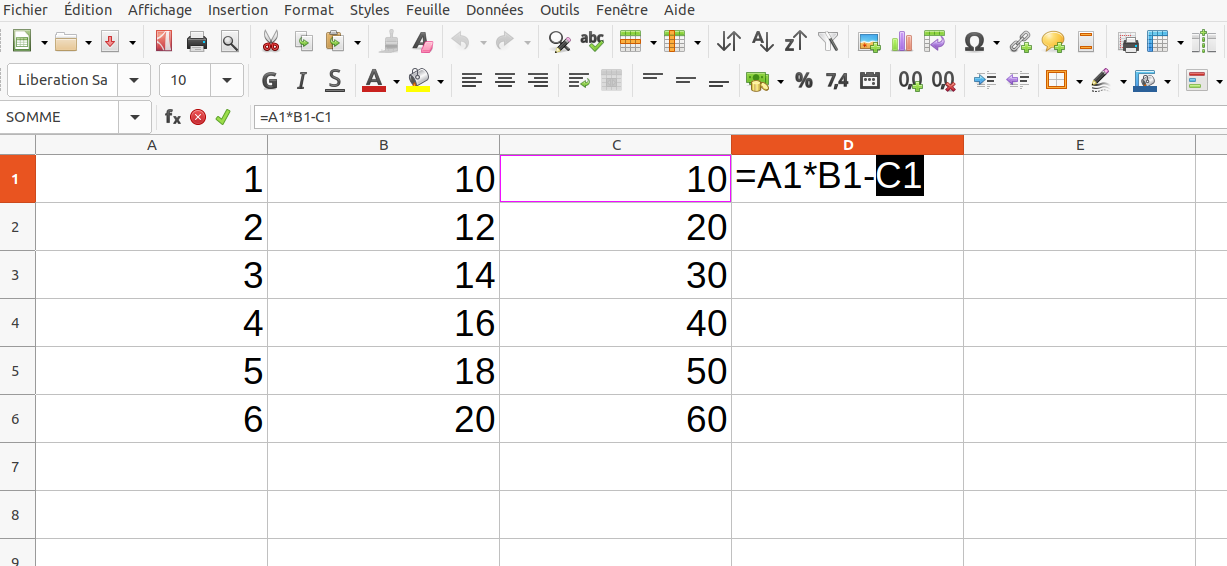
\includegraphics[width=\linewidth]{4x2-proportionnalite/ie-tableur.png}
  \end{figure}

\end{minipage}

\begin{enumerate}
  \item[3.] Quel nombre sera affiché dans la case \textbf{C7} après avoir \textbf{étiré} le tableau vers le bas ? \dotfill
  \item[4.] Quel nombre sera affiché dans la case \textbf{D3} après avoir \textbf{étiré} la formule de la case D1 ? \dotfill
  \item[5.] Quelle formule écrire dans la case \textbf{E2} pour faire le calcul : $(20-12) \times 2$ ? \dotfill
\end{enumerate}

\newpage

\subsection*{ex4 - Des petits problèmes}
\textit{Il faut résoudre et rédiger les problèmes suivants :} (\textbf{sur feuille})

\subsection*{pb1 - argent}
Il est possible de convertir des euros (€) en gils (G) en suivant cette règle : 7€ = 16G.
\textbf{(Faire le tableau, écrire le calcul, écrire une phrase réponse)}

\begin{enumerate}
  \item[1.] Vincent souhaite acheter une jolie cape. Elle coûte 325G. Quel est son prix en euros ? 
  \item[2.] Barret souhaite plutôt acheter un gilet. Il possède 63€. Quel prix maximal peut-il y mettre en gils ?
\end{enumerate}

\subsection*{pb2 - Recette}
Voici la recette d'un gratin de patates pour \textbf{5 personnes}. 

\begin{minipage}[t]{0.45\textwidth}
  \textbf{Ingrédients : }
  \begin{itemize}
    \item 1,2 kg de patates.
    \item 100 g de fromage râpé.
    \item 50 ml de lait.
    \item 40g de crème fraîche.
  \end{itemize}

\end{minipage}
\begin{minipage}[t]{0.5\textwidth}
  \textbf{Recette :}
  \begin{itemize}
    \item Éplucher les patates et les couper en fines rondelles.
    \item Mélanger le lait et la crème dans un saladier et faites tremper les rondelles de patates dedans.
    \item Disposer des couches successives de rondelles de patates dans un plat à gratin. 
    \item Faire cuire au four pendant 1h, thermostat 7.
  \end{itemize}
\end{minipage}

\begin{enumerate}
  \item[1.] On souhaite adapter la quantité d'ingrédient à \textbf{12 personnes.} \textbf{(Faire le tableau, écrire les calculs, écrire une liste réponse)}
  \item[2.] Va-t-on changer la température du four pour cette cuisson pour 12 personnes ?  \textbf{(Écrire une phrase réponse)}
  \item[3.] Un thermostat de four est proportionnel à la température. On donne thermostat 1 = 30°C. Quelle est la température du four thermostat 7. \textbf{(Écrire le calcul, écrire une phrase réponse)} 
\end{enumerate}

\end{document}